%%%%%%%%%%%%%%%%%%%%%%%%
%
% $Autor: Wings $
% $Datum: 2020-07-24 09:05:07Z $
% $Pfad: GDV/Vortraege/latex - Ausarbeitung/Kapitel/Einleitung.tex $
% $Version: 4732 $
%
%%%%%%%%%%%%%%%%%%%%%%%%

\chapter{Introduction}

\section{Introduction into your case for demonstrating of your analytics, if not given define one use case}

\subsection{Describe your case}

The systematic examination of a person's walking gait is known as gait analysis. Examining a person's gait is crucial for spotting anomalies in their walking style \cite{Hannink2016}. Changes in gait patterns provide vital fitness information that might be utilized to evaluate or analyze people suffering from pathological conditions that affect their capacity to walk and their entire bio-mechanics system \cite{Ahmadi2016}. Gait analysis was once performed by a human observer, however and video recording has made the process more reliable and precise. This qualitative analysis method is still widely known. But, this method is labor-intensive, requires an expert therapist, and requires more precision than motion analysis.

\bigskip

Hence, a more objective gait technique is required, and an \ac{imu} is another viable solution for the previously mentioned study. The use of IMU sensors with accelerometers has already been employed as an ambulatory monitoring solution for gait analysis, e.g.,\cite{Godfrey2008},\cite{Selles2005},\cite{Sabatini2005}. In addition, medical professionals can use this instrument to evaluate kinematic gait parameters throughout several steps and for a predetermined amount of time. There are a wide variety of clinical uses for the gait analysis system. Tools are used to rehabilitate and diagnose medical conditions and sports activities. 

\bigskip

Therefore, we conducted the research and looked into the usefulness of a gait pattern using an Arduino Portenta H7 IMU, specifically an accelerometer. Furthermore, we will look into how a \ac{rnn} can be used to predict gait injury from the data provided by the Arduino Portenta H7 IMU. The following sections will provide more in-depth coverage of the topics introduced earlier.

\subsection{What are the challenge and which results are reached?}

The most challenging aspects of this research are including describing the recording method, determining how speed should be represented based on gait terminology, and analyzing how the feet move while walking. All three of these tasks are interconnected.

\bigskip

A. It is challenging to employ an Arduino Portenta H7 IMU sensor equipped with an accelerometer to address the recolonization of the gait pattern due to the abundance of potential attachment spots. The body plane is another crucial feature that must be considered. It is not just the microcontroller itself, but the whole system, including the battery and how it communicates with the compiler (Cable, Infrared, Bluetooth, etc.)

\bigskip

B. Speed is the rate of change in any object's position. It is also a ratio between distance covered and time. In gates terminology, speed is the time needed to cover a short distance on flat ground. Consequently, it is difficult for us to determine the required distance and time. In addition, one must comprehend how accelerometers function because they measure in either meter per second squared ($m/s^2$) or G-forces ($g$). Consideration of their mathematical relationship presents us with a further obstacle.


\bigskip

C. Before working with sensor data, we must first analyze gait patterns, or feet's movement, to know which data and format to use. The goal is to use wavelet-based approaches to analyze accelerometer data and define the gait cycle stages. After that, we must examine speed, periodicity, and strength. Also, consider the body plane.

\section{Positioning your Analytic in front of existing solution}
\label{chapter:Positioning your Analytic in front of existing solution}

Machine learning techniques typically consist of two main components after pre-processing the motion data include Feature extraction from the input signal in brief windows of the streaming data and Model training to construct a predictive model fed by the data at the feature space.

\bigskip

Gait recognition applications have made use of a wide range of modeling algorithms, including Bayesian network classifier \cite{Kwapisz2010}, hidden Markov model classifier \cite{Rong2007}, support vector machines \cite{Kwapisz2010}, and decision trees \cite{Kwapisz2010}. The quality of these systems' predictions depends on the features used to build the hypothesis class. Noise and motion artifacts make it hard to extract important features from complex sensor data.

\bigskip

Due to the complexity of IMU sensor data, collecting manual features for machine learning-based systems is time-consuming, subjective, and prone to biases. Manual feature extraction can lead to poor feature set expressivity (i.e., the possible predictors with a fixed set of features may need to be better). Given the manual characteristics, the best model may have lower accuracy than the ideal performance in the representative feature subspace. Separating feature extraction and predictive model training also reduces machine learning-based methods' expressivity. In this approach, critical information for high-performance predictive modeling should be extracted.

\pagebreak

\bigskip

Nonetheless, this motivates us to investigate other algorithms based on wearable equipment that supply more precision for gait recognition \cite{Dehzangi2017}, including the prediction function. One study as shown in Figure \ref{fig:The overview of existing system for Human Gait Identification} provides a novel approach to human gait identification by using \ac{tf} expansion of human gait cycles to capture joint 2-dimensional (2D) spectral and temporal characteristics of gait cycles. Construct a \ac{dcnn} model that is optimized for discriminative purposes by training for each of the sensor nodes (i.e., five inertial sensors) and the modalities (i.e., accelerometer and Gyroscope readings) to extract unique signature patterns from the 2D expanded gait cycles.

\begin{figure}[h]
    \centering
    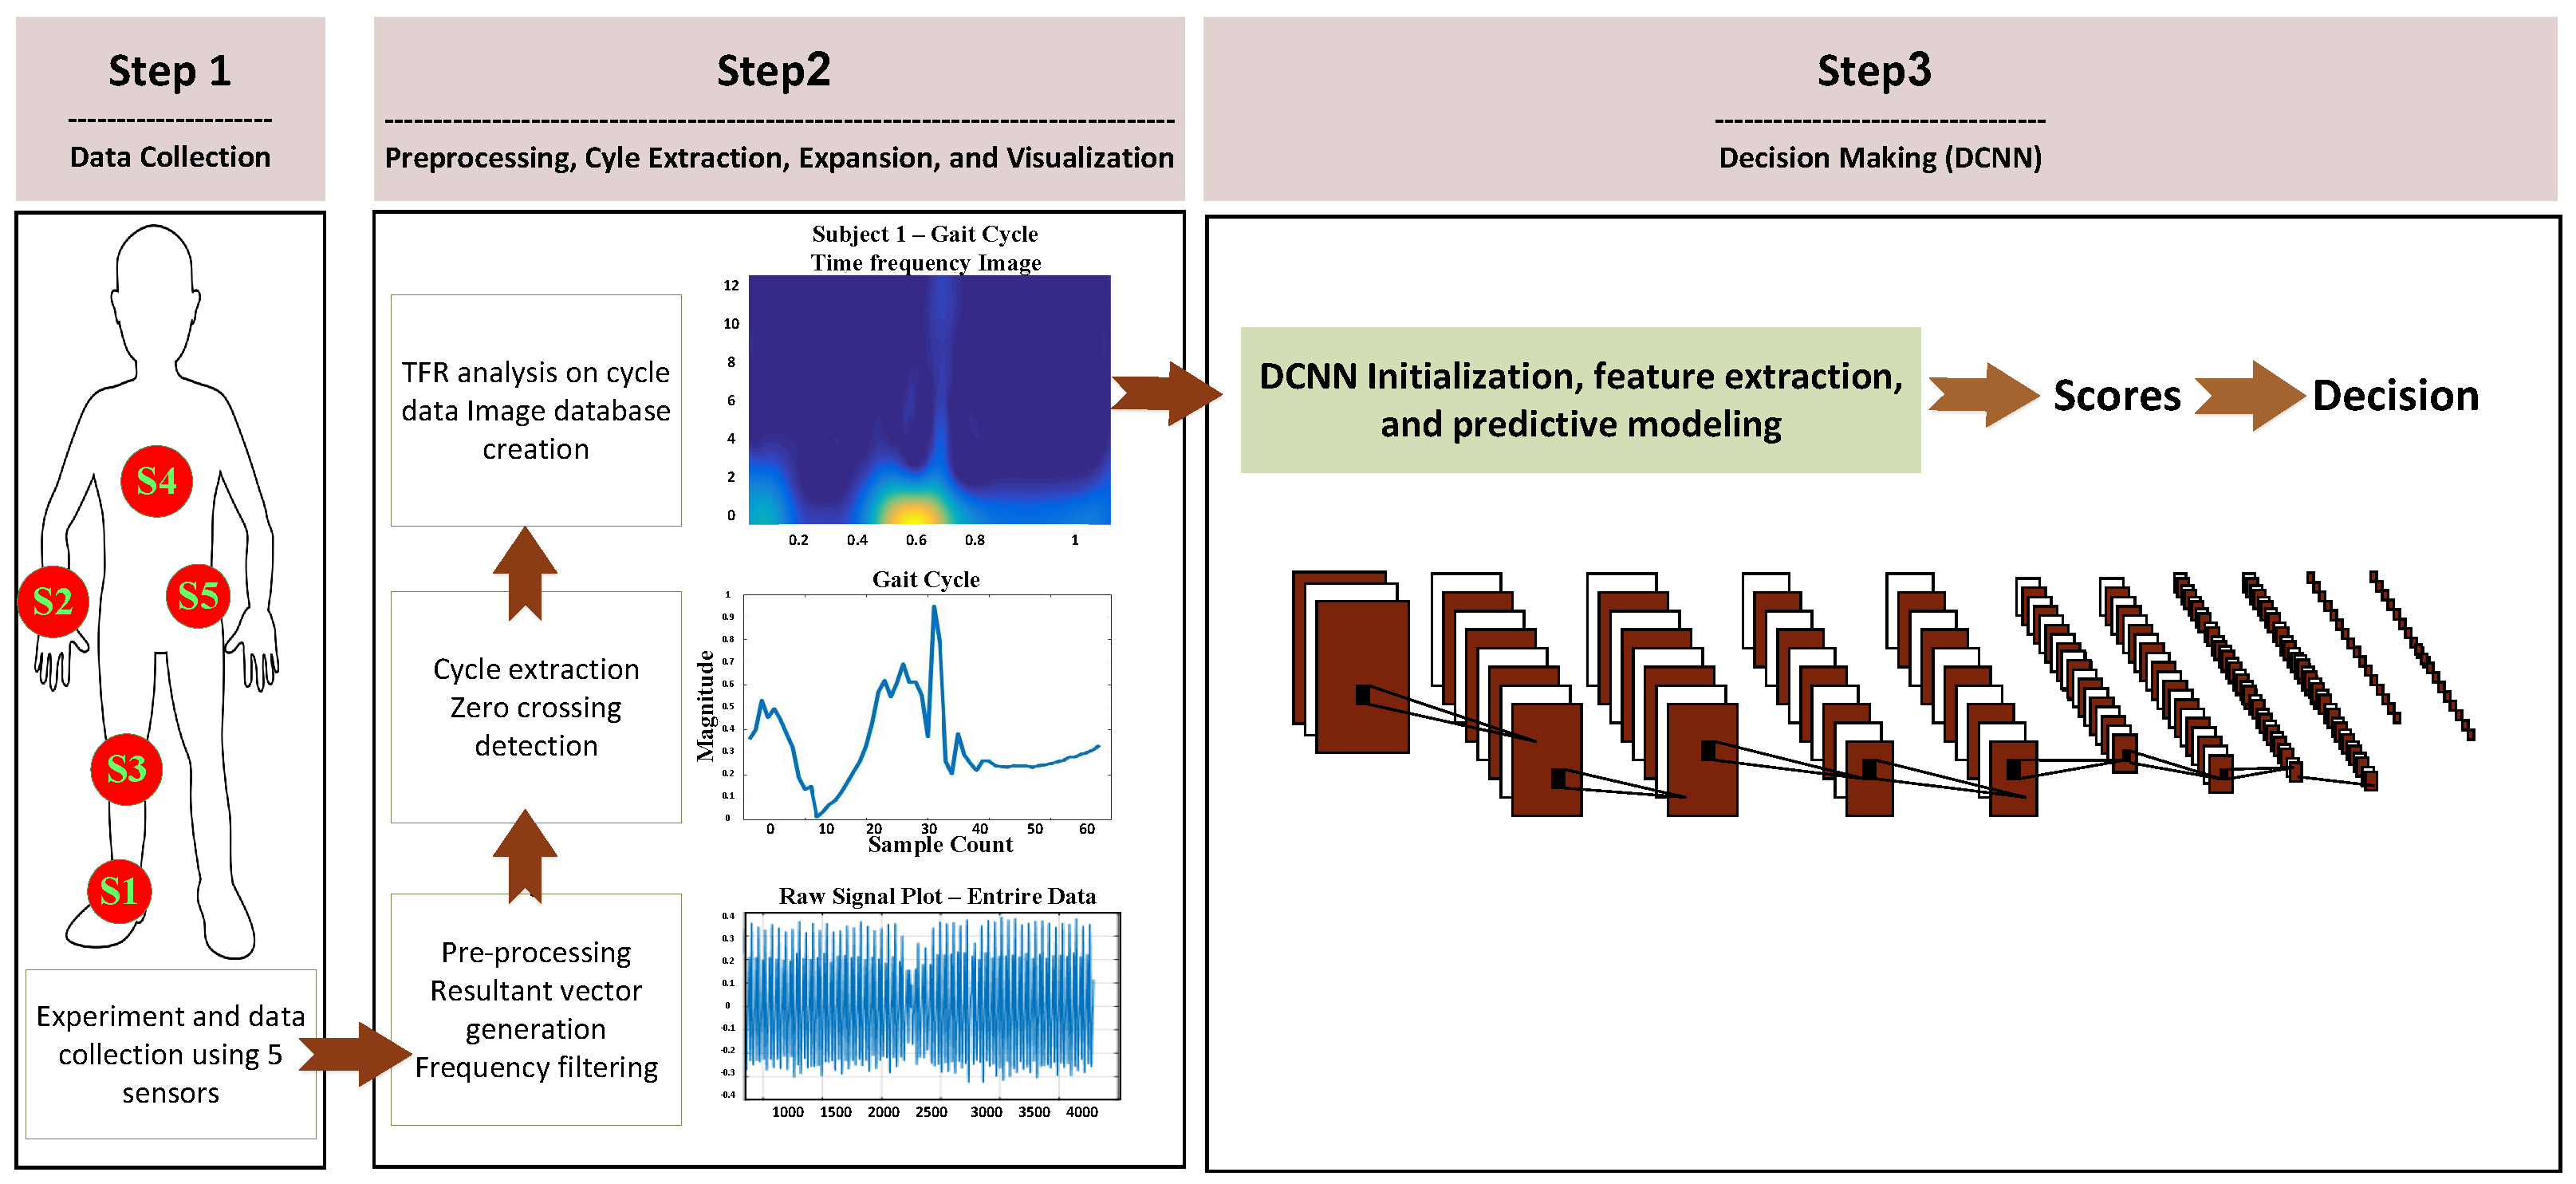
\includegraphics[scale=0.125]{Images/The overview of our existing system for Human Gait Identification.png}
    \captionsetup{justification=centering}
    \caption{The overview of existing system for Human Gait Identification \\ source: \cite{Dehzangi2017}}
    \label{fig:The overview of existing system for Human Gait Identification}
\end{figure}

\bigskip

When considering the state of the art, it could be used for the multiple application involved gait features when measured concurrently in both feet. On the other hand, Due to the fact that data from different sensors (i.e., sources) may have different characteristics, the DCNN training paradigm can be improved by sensor-dependent tuning for different sensor locations and modalities. Therefore, accuracy is not the only or primary concern for gait analysis, and other relevant shall be concerned include easily operational, less-space-consuming, non-expensive, and reliable.

\bigskip

For all of those reasons regard the disadvantage of the mentioned study, our primary objective was to identify a means of determining the gait phase that was not only more accurate but also required fewer resources and was less costly. Likewise, instead of using multiple sensors, Arduino Portenta H7 IMU shall be used to measure the acceleration of the foot. The use of a Neural Network as a model is going to be required in order to differentiate between gait phases and provide prediction in foot and ankle injuries.